\chapter{Building a Potential from the Zeros: the Wu--Sprung Construction}\label{ch:wu-sprung}

\begin{chapterintro}
Until now the arrow has pointed one way. You were handed a potential $V(x)$ and asked for its energy levels: solve $H\psi=E\psi$, find the list $E_1,E_2,\dots$. In this chapter we reverse the arrow. Someone hands you a list of numbers and asks: \emph{what potential well would have these numbers as its energy levels?} This is the \emph{inverse spectral problem}, and it is the heart of the empirical side of the Hilbert--P\'olya program you met in Chapter~\ref{ch:hilbert-polya}.

In 1993 Wu and Sprung \cite{wusprung} asked this question for the Riemann zeros. They did not try to reproduce every zero at once. They first asked for a smooth, even potential whose levels have exactly the \emph{average} spacing of the zeros, the spacing described by the smooth counting function $\Nsm$ of Chapter~\ref{ch:counting-zeros}. Using the semiclassical counting of Chapter~\ref{ch:wkb}, this question turns into an integral equation first solved by Abel, and its solution is a closed formula for the potential. We derive that formula line by line, find out where its single constant $V_0$ comes from, study the shape of the resulting well, and check numerically that its levels really do sit on the smooth zeros.

Where this shows up in the paper \cite{soniR1}: the formula we derive is the paper's Eq.~(2) in Sec.~II~B; the box half-widths $L=44.883$ and $59.957$ come from it; it is the ``smooth potential'' and the null model of every operator fit in Secs.~II~C, III and V; the turning-point map we build explains the paper's statement (Sec.~III, interpolation split) that ``position maps to level index through the classical turning point''; and the closing section explains why the whole empirical program, of which the paper is a test, needs held-out data.
\end{chapterintro}

\begin{prerequisites}
\item Chapter~\ref{ch:bound-states}: levels of the infinite well on $[-L,L]$, $E_k=(k\pi/2L)^2$; the harmonic oscillator levels $1,3,5,\dots$ for $V=x^2$ in units $\hbar=2m=1$; even potentials; slowly growing potentials have crowded levels.
\item Chapter~\ref{ch:wkb}: the local wavenumber $\sqrt{E-V(x)}$, classical turning points, Bohr--Sommerfeld quantization with the $(n-\tfrac12)\pi$ rule, the semiclassical counting function, the idea of inverting a counting function by an Abel integral equation.
\item Chapter~\ref{ch:counting-zeros}: the smooth counting function $\Nsm(t)$, the smooth zeros $s_n$, the mean spacing $\gap_n$, and fluctuations measured in mean spacings.
\item Chapter~\ref{ch:hilbert-polya}: the Hilbert--P\'olya conjecture (open), and the distinction between analytic operator proposals and empirical fits.
\item Chapter~\ref{ch:asymptotics}: big-$\mathcal O$ notation, root finding (Brent), floating-point round-off and machine epsilon; an exponential grows faster than any power.
\item Chapter~\ref{ch:schrodinger}: the Hamiltonian $H=-d^2/dx^2+V$ in units $\hbar=2m=1$ and the meaning of an energy level.
\item Chapter~\ref{ch:series}: the Taylor series of $\log(1\pm r)$.
\item Chapter~\ref{ch:eigen}: tridiagonal matrices and numerical eigensolvers used as black boxes.
\item Chapter~\ref{ch:explicit-formula}: the explicit formula, as background for the fluctuations discussed in Section~\ref{sec:wu-sprung-empirical}.
\item Chapter~\ref{ch:finite-differences} (a later chapter): its results are used once, in Section~\ref{sec:wu-sprung-check}, and are stated there explicitly as taken on trust.
\item First-year physics: potential-energy curves, turning points, energy conservation $\tfrac12 mv^2+V=E$.
\item Calculus: substitution, integration by parts, the antiderivative $z\log z-z$ of $\log z$, the fundamental theorem of calculus.
\end{prerequisites}

%======================================================================
\section{The inverse spectral problem}\label{sec:wu-sprung-inverse}

\subsection{Forward and inverse}

Recall from Chapter~\ref{ch:schrodinger} that in units $\hbar=2m=1$ the Hamiltonian of a particle on a line is
\begin{equation}
H=-\frac{d^2}{dx^2}+V(x),
\label{eq:wu-sprung-H}
\end{equation}
where $V(x)$ is the potential energy, and that an energy level $E$ is a number for which $H\psi=E\psi$ has a normalizable solution $\psi$. In these units an energy and a ``height'' $t$ on the critical line are measured in the same way, which is why we can compare levels $E_n$ directly with zeros $t_n$.

The \textbf{forward problem} is: given $V$, find the levels. The \textbf{inverse spectral problem} is: given the levels, find $V$. You have a physical feel for the inverse problem already. A trained ear can tell a large bell from a small one, or a steel drum from a timpani, from the frequencies alone. In 1966 the mathematician Mark Kac popularized the question ``Can one hear the shape of a drum?'', asking whether the frequencies of a drumhead determine its outline.

For us the ``drum'' is a one-dimensional well and the ``frequencies'' are the levels. The first lesson of the inverse problem is that the answer is usually \emph{not unique}, and we must decide what extra assumptions pin it down.

\subsection{Three ways to get the same spectrum}

\textbf{Translation.} On the whole line, shift the potential sideways: $\tilde V(x)=V(x-x_0)$ for a constant $x_0$. If $\psi$ solves $-\psi''(x)+V(x)\psi(x)=E\psi(x)$ for all $x$, define $\varphi(x)=\psi(x-x_0)$. By the chain rule $\varphi''(x)=\psi''(x-x_0)$, so evaluating the original equation at the point $x-x_0$ gives
\[
-\varphi''(x)+V(x-x_0)\varphi(x)=E\varphi(x).
\]
So $\tilde V$ has the same level $E$, with the same normalization (shifting does not change $\int|\varphi|^2\dd x$). Every level of $V$ is a level of $\tilde V$ and, running the argument backwards with $-x_0$, vice versa.

\textbf{Reflection.} Let $\tilde V(x)=V(-x)$ and $\varphi(x)=\psi(-x)$. Then $\varphi'(x)=-\psi'(-x)$ and $\varphi''(x)=\psi''(-x)$, so again $-\varphi''+\tilde V\varphi=E\varphi$. A well and its mirror image have the same spectrum.

\textbf{Shearing (semiclassical).} This one is less obvious and is the important one. We show next that, within the semiclassical approximation of Chapter~\ref{ch:wkb}, the levels of a single well depend on the potential only through how \emph{wide} the well is at each height, not on how that width is placed left and right.

\subsection{Slicing the well horizontally}

Consider a single well: $V$ has one minimum value $V_0$ and rises on both sides. For each height $V\ge V_0$ let $x_-(V)\le x_+(V)$ be the two points where the potential equals $V$, and define the \textbf{width function}
\begin{equation}
w(V)=x_+(V)-x_-(V),
\label{eq:wu-sprung-width-def}
\end{equation}
the length of the horizontal chord of the well at height $V$. At energy $E$ the classical turning points are $x_\pm(E)$.

Recall from Chapter~\ref{ch:wkb} the phase integral, which we call
\begin{equation}
\Phi(E)=\int_{x_-(E)}^{x_+(E)}\sqrt{E-V(x)}\,\dd x ,
\label{eq:wu-sprung-phi}
\end{equation}
and the Bohr--Sommerfeld rule: the $n$-th level $E_n$ ($n=1,2,\dots$) satisfies
\begin{equation}
\Phi(E_n)=\Bigl(n-\tfrac12\Bigr)\pi .
\label{eq:wu-sprung-bs}
\end{equation}
This is an approximation (Chapter~\ref{ch:wkb}): accurate for high levels, weaker for the lowest few.

Now the trick. For a fixed $x$ inside the well, write the square root as an integral over heights:
\begin{equation}
\sqrt{E-V(x)}=\int_{V(x)}^{E}\frac{\dd V'}{2\sqrt{E-V'}} .
\label{eq:wu-sprung-sqrt-int}
\end{equation}
Check it with the fundamental theorem of calculus: an antiderivative of $1/(2\sqrt{E-V'})$ with respect to $V'$ is $-\sqrt{E-V'}$; evaluated between $V(x)$ and $E$ it gives $0-\bigl(-\sqrt{E-V(x)}\bigr)=\sqrt{E-V(x)}$. The integrand blows up at $V'=E$, but only like an inverse square root, and the integral is finite (it equals a square root), so nothing is wrong.

Put \eqref{eq:wu-sprung-sqrt-int} into \eqref{eq:wu-sprung-phi}:
\begin{equation}
\Phi(E)=\int_{x_-(E)}^{x_+(E)}\left[\int_{V(x)}^{E}\frac{\dd V'}{2\sqrt{E-V'}}\right]\dd x .
\label{eq:wu-sprung-double}
\end{equation}
Read this as a sum over tiny rectangles of size $\dd x\times\dd V'$ in the $(x,V')$ plane, each carrying the weight $1/(2\sqrt{E-V'})$. Which rectangles? Those with $x$ between the turning points and $V'$ between the floor $V(x)$ and the ceiling $E$: that is, exactly the region \emph{inside the well and below the energy} $E$ (the shaded region you would draw on a potential-energy diagram from first-year physics). We have added up this region in vertical strips: first up a column at fixed $x$, then across all columns.

We can add the same rectangles in horizontal strips instead: first along a row at fixed height $V'$, then up all rows from $V_0$ to $E$. At fixed height $V'$ the row runs over the $x$ where $V(x)\le V'$, which for a single well is the interval $[x_-(V'),x_+(V')]$ of length $w(V')$. The weight does not depend on $x$, so the row contributes $w(V')/(2\sqrt{E-V'})\,\dd V'$, and
\begin{equation}
\boxed{\;\Phi(E)=\int_{V_0}^{E}\frac{w(V)}{2\sqrt{E-V}}\,\dd V\;}
\label{eq:wu-sprung-width}
\end{equation}
(we renamed $V'$ to $V$).

\begin{beyond}
\textbf{Swapping the order of integration.} We used the fact that adding up a positive weight over a region gives the same answer whether you sum columns first or rows first. For positive integrands this is a theorem of measure theory (Tonelli's theorem), valid even when the weight has an integrable singularity on the boundary as ours does at $V=E$. Double integrals and changes of order are treated in Riley, Hobson and Bence \cite{rhb}. We take the theorem on trust; nothing in this chapter needs more than ``rows-first equals columns-first for a positive weight''.
\end{beyond}

Equation~\eqref{eq:wu-sprung-width} says something remarkable: \emph{the phase integral, and hence every Bohr--Sommerfeld level, depends on the well only through its width function $w(V)$}. Two wells with the same chord length at every height have the same semiclassical spectrum, however the chords are slid left or right. \Cref{fig:wu-sprung-nonunique} shows an example.

\begin{figure}[htbp]\centering
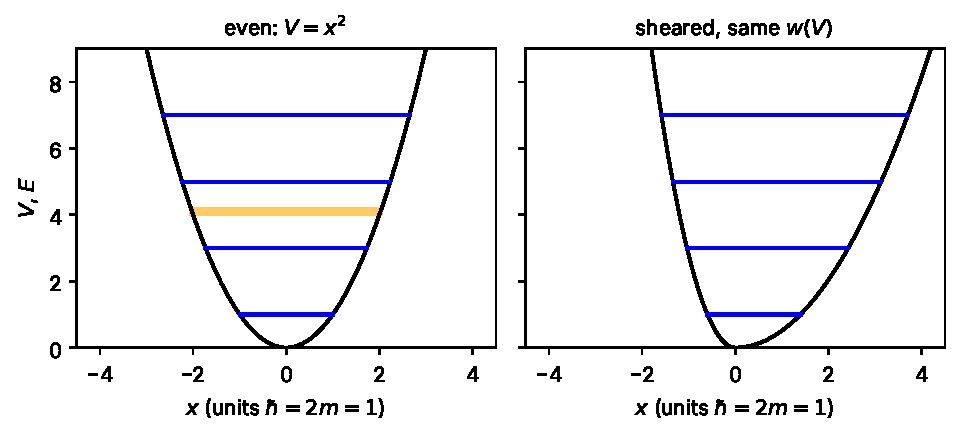
\includegraphics[width=0.85\linewidth]{figs/wu-sprung_nonunique.pdf}
\caption{Two single wells with the same width function $w(V)=2\sqrt V$. Left: the even harmonic well $V=x^2$. Right: a ``sheared'' well with $x_+(V)=1.4\sqrt V$ and $x_-(V)=-0.6\sqrt V$, so it is steep on the left and gentle on the right. Horizontal segments are the Bohr--Sommerfeld levels $E=1,3,5,7$ drawn between their turning points; they are identical in both panels because each chord has the same length. The shaded strip in the left panel is one horizontal slice of height $\dd V$ used in Eq.~\eqref{eq:wu-sprung-width}. Units $\hbar=2m=1$.}
\label{fig:wu-sprung-nonunique}
\end{figure}

\begin{sample}{A lopsided oscillator with an ordinary spectrum}
Take $0<\beta<1$ and the potential $V(x)=x^2/(1+\beta)^2$ for $x\ge0$ and $V(x)=x^2/(1-\beta)^2$ for $x<0$. Find its Bohr--Sommerfeld levels.

\textbf{Step 1: turning points.} For $x\ge0$, $V=x^2/(1+\beta)^2$ gives $x_+(V)=(1+\beta)\sqrt V$. For $x<0$, $V=x^2/(1-\beta)^2$ gives $x_-(V)=-(1-\beta)\sqrt V$.

\textbf{Step 2: width.} $w(V)=x_+-x_-=(1+\beta)\sqrt V+(1-\beta)\sqrt V=2\sqrt V$, independent of $\beta$.

\textbf{Step 3: compare.} For $\beta=0$ the potential is $V=x^2$, whose width is also $2\sqrt V$. By Eq.~\eqref{eq:wu-sprung-width} the two wells have the same $\Phi(E)$ for every $E$, and therefore the same Bohr--Sommerfeld levels. For $V=x^2$ these are $E_n=2n-1$ (we verify this in the next section's Sample Problem).

\[
\boxed{E_n=2n-1\ \text{ for every }0\le\beta<1\ \text{(semiclassically)}}
\]
The exact quantum levels of the lopsided well need not equal $2n-1$; the statement is about the semiclassical spectrum.
\end{sample}

\subsection{Fixing the ambiguity: even and monotone}

Since the semiclassical spectrum determines only $w(V)$, we must add assumptions to get a single answer. The natural ones are:
\begin{enumerate}
\item \textbf{Evenness}, $V(-x)=V(x)$. Then $x_-(V)=-x_+(V)$. Writing $x(V)\equiv x_+(V)$ we get $w(V)=2x(V)$, so knowing $w$ means knowing $x(V)$. Evenness also removes translation (the well is centered at $0$) and reflection (the mirror image is the same well).
\item \textbf{Monotonicity}: $V$ increases for $x>0$. Then the well is a single well, each height $V$ is reached at exactly one positive $x$, and $x(V)$ is a genuine function, the inverse of $V(x)$ on $x\ge0$.
\end{enumerate}
With both assumptions, Eq.~\eqref{eq:wu-sprung-width} becomes
\begin{equation}
\boxed{\;\Phi(E)=\int_{V_0}^{E}\frac{x(V)}{\sqrt{E-V}}\,\dd V\;}
\label{eq:wu-sprung-layer}
\end{equation}
This is the equation we must solve: $\Phi(E)$ is prescribed by the levels we want, and $x(V)$ is unknown.

\begin{beyond}
\textbf{The exact (non-semiclassical) inverse problem.} Even when the spectrum is computed exactly rather than by WKB, a single spectrum does not in general determine a potential: there exist distinct ``isospectral'' potentials. A classical theorem of G.~Borg (1946) states that for a potential on a finite interval with Dirichlet ends that is symmetric about the midpoint, the spectrum does determine the potential uniquely. We do not use this theorem; the Wu--Sprung construction is semiclassical from the start. It is mentioned only so that you know evenness is the right kind of extra assumption in the exact theory as well.
\end{beyond}

\begin{checkpoint}
A friend claims to have measured the first 200 levels of a single-well potential to great accuracy, and to have deduced from them that the well is steeper on the left than on the right. Within the semiclassical approximation, can the levels support that claim?
\end{checkpoint}
\checkanswer{No. Semiclassically the levels depend only on the width $w(V)$ (Eq.~\eqref{eq:wu-sprung-width}); any redistribution of each chord between left and right leaves them unchanged. The asymmetry claim needs information beyond the levels, for example an assumption or a measurement of the wavefunctions.}

\begin{keyideas}
\item The inverse spectral problem (levels $\to$ potential) has non-unique answers: translation, reflection, and, semiclassically, any shear that preserves chord lengths.
\item Slicing the well horizontally gives $\Phi(E)=\int_{V_0}^{E}w(V)\,\dd V/(2\sqrt{E-V})$, Eq.~\eqref{eq:wu-sprung-width}: WKB levels see only the width function.
\item Assuming an even, monotone single well fixes $w=2x(V)$ and gives the integral equation \eqref{eq:wu-sprung-layer} for the unknown $x(V)$.
\end{keyideas}

%======================================================================
\section{The target: a level density that grows like a logarithm}\label{sec:wu-sprung-target}

\subsection{What the zeros ask for, on average}

Recall from Chapter~\ref{ch:counting-zeros} the smooth counting function of the Riemann zeros, the paper's Eq.~(1):
\begin{equation}
\Nsm(t)=\frac{t}{2\pi}\log\frac{t}{2\pi}-\frac{t}{2\pi}+\frac78 ,
\label{eq:wu-sprung-nsm}
\end{equation}
where $\log$ is the natural logarithm. It describes the \emph{average} number of nontrivial zeros $\rho_n=\tfrac12+it_n$ with height $0<t_n\le t$. Recall also the \textbf{smooth zeros} $s_n$, defined by
\begin{equation}
\Nsm(s_n)=n-\tfrac12 ,
\label{eq:wu-sprung-sn}
\end{equation}
which are where the zeros would sit if there were no fluctuations, and the \textbf{local mean spacing} $\gap_n=\dd s_n/\dd n$.

Differentiate \eqref{eq:wu-sprung-nsm} with the product rule. The first term gives $\frac{1}{2\pi}\log\frac{t}{2\pi}+\frac{t}{2\pi}\cdot\frac1t$, the second gives $-\frac1{2\pi}$, the constant gives $0$:
\begin{equation}
\Nsm'(t)=\frac{1}{2\pi}\log\frac{t}{2\pi}+\frac1{2\pi}-\frac1{2\pi}=\frac{1}{2\pi}\log\frac{t}{2\pi}.
\label{eq:wu-sprung-nsmprime}
\end{equation}
$\Nsm'(t)$ is the \textbf{level density}: the average number of zeros per unit height. Differentiating \eqref{eq:wu-sprung-sn} with respect to $n$ gives $\Nsm'(s_n)\,\dd s_n/\dd n=1$, so
\begin{equation}
\gap_n=\frac{1}{\Nsm'(s_n)}=\frac{2\pi}{\log(s_n/2\pi)} .
\label{eq:wu-sprung-gap}
\end{equation}

\begin{sample}{Density and spacing at height 1000}
Find the level density and the mean spacing of the zeros at $t=1000$, and the smooth number of zeros below $1000$.

\textbf{Step 1:} $1000/2\pi=159.155$ and $\log 159.155=5.0699$.

\textbf{Step 2:} By \eqref{eq:wu-sprung-nsmprime}, $\Nsm'(1000)=5.0699/(2\pi)=0.8069$ zeros per unit height.

\textbf{Step 3:} By \eqref{eq:wu-sprung-gap}, the spacing is $1/0.8069=2\pi/5.0699=1.239$.

\textbf{Step 4:} By \eqref{eq:wu-sprung-nsm}, $\Nsm(1000)=159.155\times5.0699-159.155+0.875=648.6$.

\[
\boxed{\Nsm'(1000)\approx0.807,\qquad \gap\approx1.239,\qquad \Nsm(1000)\approx648.6}
\]
The density \emph{increases} slowly with height (like a logarithm), so the zeros crowd together slowly as you go up.
\end{sample}

\subsection{Which wells have growing level density?}

Recall from Chapter~\ref{ch:bound-states} that the spacing of levels depends on how fast the potential rises. Let us make that quantitative for the power-law family $V(x)=|x|^\alpha$ with $\alpha>0$.

\begin{sample}{Phase integrals of power-law wells}
Compute $\Phi(E)$ for $V=|x|^\alpha$, then specialize to the harmonic ($\alpha=2$) and linear ($\alpha=1$) wells and find their Bohr--Sommerfeld levels.

\textbf{Step 1: turning points.} $|x|^\alpha=E$ gives $x_\pm=\pm E^{1/\alpha}$.

\textbf{Step 2: use evenness.} $\Phi(E)=2\int_0^{E^{1/\alpha}}\sqrt{E-x^\alpha}\,\dd x$.

\textbf{Step 3: scale out $E$.} Substitute $x=E^{1/\alpha}u$, so $\dd x=E^{1/\alpha}\dd u$ and $E-x^\alpha=E(1-u^\alpha)$:
\[
\Phi(E)=2\int_0^1\sqrt{E}\sqrt{1-u^\alpha}\;E^{1/\alpha}\dd u=2E^{\frac12+\frac1\alpha}I_\alpha,\qquad I_\alpha=\int_0^1\sqrt{1-u^\alpha}\,\dd u .
\]

\textbf{Step 4: harmonic.} $I_2=\int_0^1\sqrt{1-u^2}\,\dd u$ is the area of a quarter of the unit disk, $\pi/4$. So $\Phi=2E\cdot\pi/4=\pi E/2$. Bohr--Sommerfeld \eqref{eq:wu-sprung-bs}: $\pi E_n/2=(n-\tfrac12)\pi$, so $E_n=2n-1$. These are exactly the oscillator levels $1,3,5,\dots$ of Chapter~\ref{ch:bound-states}.

\textbf{Step 5: linear.} $I_1=\int_0^1(1-u)^{1/2}\dd u=\bigl[-\tfrac23(1-u)^{3/2}\bigr]_0^1=\tfrac23$. So $\Phi=\tfrac43E^{3/2}$ and $E_n=\bigl[\tfrac{3\pi}{4}(n-\tfrac12)\bigr]^{2/3}$.

\[
\boxed{\Phi(E)=2I_\alpha E^{\frac12+\frac1\alpha};\quad \alpha=2:\ E_n=2n-1;\quad \alpha=1:\ E_n=\Bigl[\tfrac{3\pi}{4}\bigl(n-\tfrac12\bigr)\Bigr]^{2/3}}
\]
\end{sample}

By Bohr--Sommerfeld the smooth number of levels below $E$ is $\Phi(E)/\pi$ up to a constant, so for $|x|^\alpha$ it grows like $E^{1/2+1/\alpha}$, and the level density $\dd(\Phi/\pi)/\dd E$ grows like $E^{1/\alpha-1/2}$:
\begin{itemize}
\item $\alpha>2$ (steeper than harmonic; the box is $\alpha\to\infty$): density falls, levels spread apart;
\item $\alpha=2$: constant density, equally spaced levels;
\item $\alpha<2$ (softer than harmonic): density grows, levels crowd together.
\end{itemize}
The zeros have a density that grows, but only logarithmically, Eq.~\eqref{eq:wu-sprung-nsmprime}. So we should expect a potential that is softer than harmonic, though not by a fixed power. We will see in Section~\ref{sec:wu-sprung-shape} what the answer actually looks like.

\begin{pitfall}
Do not confuse ``a potential that grows slowly'' with ``levels that are far apart''. It is the opposite: a slowly growing potential is a wide well at high energy, and wide wells have closely spaced levels (think of the box: doubling $L$ quarters the levels). Soft wells crowd their levels.
\end{pitfall}

\subsection{The matching condition}

Here is the precise demand. Put side by side the two equations that define the two lists of numbers:
\[
\text{Bohr--Sommerfeld: }\ \frac{\Phi(E_n)}{\pi}=n-\tfrac12,\qquad\qquad \text{smooth zeros: }\ \Nsm(s_n)=n-\tfrac12 .
\]
Both have the form ``a smooth increasing function equals $n-\tfrac12$''. If the two functions are equal,
\begin{equation}
\boxed{\;\Phi(E)=\pi\,\Nsm(E)\quad\text{for all }E\ge V_0,\;}
\label{eq:wu-sprung-match}
\end{equation}
then $E_n=s_n$ for every $n$. Strictly, we only need agreement at the discrete points $s_n$; demanding it for all $E$ is our choice of the smoothest interpolation, with no wiggles between levels.

\begin{pitfall}
\textbf{Two half-integer conventions.} Chapter~\ref{ch:wkb} wrote the semiclassical counting function as $N(E)=\Phi(E)/\pi+\tfrac12$, a curve that passes through the integer $n$ at the level $E_n$. The paper's $\Nsm$ passes through $n-\tfrac12$ at $s_n$, the midpoint of the jump of the true staircase (Chapter~\ref{ch:counting-zeros}). The two conventions differ by exactly $\tfrac12$. If you set $N(E)=\Nsm(E)$ instead of \eqref{eq:wu-sprung-match} you would shift every level by half a spacing. Matching the two quantization conditions directly, as above, avoids the trap.
\end{pitfall}

Notice what Eq.~\eqref{eq:wu-sprung-match} asks for and what it does not. It asks for levels at the \emph{smooth} zeros $s_n$, not at the true zeros $t_n$. The potential we are about to build knows the average spacing of the zeros and nothing about their individual fluctuations.

\begin{checkpoint}
Below $t=2\pi$, Eq.~\eqref{eq:wu-sprung-nsmprime} gives a negative level density. Should this worry us?
\end{checkpoint}
\checkanswer{Not much. $\Nsm$ is an asymptotic description of the zeros for large $t$ (Chapter~\ref{ch:counting-zeros}); the first zero is at $t_1=14.13$, well above $2\pi\approx6.28$. But it does tell us the well must start above $2\pi$; we make this precise in Section~\ref{sec:wu-sprung-v0}.}

\begin{keyideas}
\item The zeros' level density is $\Nsm'(t)=\frac{1}{2\pi}\log\frac{t}{2\pi}$, Eq.~\eqref{eq:wu-sprung-nsmprime}, and their mean spacing is $\gap=2\pi/\log(t/2\pi)$, Eq.~\eqref{eq:wu-sprung-gap}.
\item Power-law wells $|x|^\alpha$ have level density $\propto E^{1/\alpha-1/2}$; a growing density needs a potential softer than harmonic.
\item The Wu--Sprung requirement is $\Phi(E)=\pi\Nsm(E)$, Eq.~\eqref{eq:wu-sprung-match}, which puts the Bohr--Sommerfeld levels on the smooth zeros $s_n$.
\end{keyideas}

%======================================================================
\section{Solving the Abel equation}\label{sec:wu-sprung-abel}

\subsection{The equation and its inversion}

Combining \eqref{eq:wu-sprung-layer} and \eqref{eq:wu-sprung-match} we must find $x(V)$ from
\begin{equation}
\int_{V_0}^{E}\frac{x(V)}{\sqrt{E-V}}\,\dd V=\Phi(E)\qquad(E\ge V_0),
\label{eq:wu-sprung-abel}
\end{equation}
with $\Phi$ given. Because the unknown sits inside an integral, this is an \emph{integral equation}. Equations with the kernel $1/\sqrt{E-V}$ are called \textbf{Abel equations}, after N.~H.~Abel, who met one in 1823 while finding the shape of a slide down which a bead takes the same time from any starting height. You met the inversion in Chapter~\ref{ch:wkb}; we redo it here in full, in exactly the form we need.

\textbf{Step A: multiply and integrate.} Pick a height $W>V_0$. Multiply \eqref{eq:wu-sprung-abel} by $1/\sqrt{W-E}$ and integrate over $E$ from $V_0$ to $W$. Call the result $J(W)$:
\begin{equation}
J(W)\equiv\int_{V_0}^{W}\frac{\Phi(E)}{\sqrt{W-E}}\,\dd E=\int_{V_0}^{W}\left[\int_{V_0}^{E}\frac{x(V)\,\dd V}{\sqrt{E-V}}\right]\frac{\dd E}{\sqrt{W-E}} .
\label{eq:wu-sprung-J}
\end{equation}

\textbf{Step B: swap the order.} The double integral runs over the triangle $V_0\le V\le E\le W$ in the $(V,E)$ plane, with the positive weight $x(V)/\sqrt{(E-V)(W-E)}$ (positive because $x(V)\ge0$). Summing rows first instead of columns first (the swap justified in Section~\ref{sec:wu-sprung-inverse}): for fixed $V$, $E$ runs from $V$ to $W$. So
\begin{equation}
J(W)=\int_{V_0}^{W}x(V)\,K(V,W)\,\dd V,\qquad K(V,W)=\int_{V}^{W}\frac{\dd E}{\sqrt{(W-E)(E-V)}} .
\label{eq:wu-sprung-K}
\end{equation}

\textbf{Step C: the kernel integral is $\pi$.} Substitute $E=V+(W-V)\sin^2\varphi$ with $0\le\varphi\le\pi/2$. Then
\begin{align*}
E-V&=(W-V)\sin^2\varphi,\\
W-E&=(W-V)(1-\sin^2\varphi)=(W-V)\cos^2\varphi,\\
\dd E&=2(W-V)\sin\varphi\cos\varphi\,\dd\varphi,\\
\sqrt{(W-E)(E-V)}&=(W-V)\sin\varphi\cos\varphi\quad\text{(both factors are }\ge0\text{ on }[0,\pi/2]).
\end{align*}
The integrand becomes $2\,\dd\varphi$, and $\varphi$ runs from $0$ (at $E=V$) to $\pi/2$ (at $E=W$):
\begin{equation}
K(V,W)=\int_0^{\pi/2}2\,\dd\varphi=\pi,
\label{eq:wu-sprung-Kpi}
\end{equation}
independent of $V$ and $W$. You can check this numerically with the short listing below. It evaluates $K(2,5)$ by adaptive quadrature, and the printed value agrees with $\pi=3.14159265\ldots$ to better than $10^{-9}$.
\begin{pycode}
import numpy as np
from scipy.integrate import quad
V, W = 2.0, 5.0
K = quad(lambda E: 1/np.sqrt((W-E)*(E-V)), V, W)[0]
print(K, np.pi)     # the two numbers agree
\end{pycode}

\textbf{Step D: undo the integral.} With $K=\pi$, Eq.~\eqref{eq:wu-sprung-K} reads $J(W)=\pi\int_{V_0}^{W}x(V)\,\dd V$. By the fundamental theorem of calculus,
\begin{equation}
x(W)=\frac1\pi\,\frac{\dd J}{\dd W}.
\label{eq:wu-sprung-xJ}
\end{equation}

\textbf{Step E: compute $\dd J/\dd W$.} The integrand of $J$ blows up at $E=W$, which makes direct differentiation awkward. Remove the singularity first: in \eqref{eq:wu-sprung-J} substitute $E=W-u^2$ with $u\ge0$. Then $\sqrt{W-E}=u$, $\dd E=-2u\,\dd u$, $E=V_0$ corresponds to $u=\sqrt{W-V_0}$ and $E=W$ to $u=0$:
\[
J(W)=\int_{u=\sqrt{W-V_0}}^{0}\frac{\Phi(W-u^2)}{u}(-2u)\,\dd u=\int_0^{\sqrt{W-V_0}}2\,\Phi(W-u^2)\,\dd u .
\]
Now the integrand is smooth. We need one piece of notation from multivariable calculus. For a function $f(u,W)$ of two variables, the \emph{partial derivative} $\partial f/\partial W$ is the ordinary derivative with respect to $W$ while $u$ is held fixed. For example, if $f(u,W)=2\Phi(W-u^2)$, then holding $u$ fixed and using the chain rule gives $\partial f/\partial W=2\Phi'(W-u^2)$. Leibniz's rule for a variable upper limit $g(W)$ says: if $f$ and $\partial f/\partial W$ are continuous, then
\[
\frac{\dd}{\dd W}\int_0^{g(W)}f(u,W)\,\dd u=f\bigl(g(W),W\bigr)\,g'(W)+\int_0^{g(W)}\frac{\partial f}{\partial W}\,\dd u .
\]
The first term is the fundamental theorem of calculus combined with the chain rule: it accounts for moving the upper limit. The second term accounts for the change of the integrand with the limits held fixed.
\begin{beyond}
\textbf{Differentiation under the integral sign.} That the change of the integrand at fixed limits contributes $\int\partial f/\partial W\,\dd u$ (that is, that one may differentiate inside the integral) is a theorem of analysis that needs the continuity hypotheses just stated. A proof is in Riley, Hobson and Bence \cite{rhb}. We take it on trust.
\end{beyond}
Are the hypotheses met? For the harmonic test below, $\Phi'$ is a constant. For the Riemann target, $\Phi'(E)=\tfrac12\log(E/2\pi)$ (Eq.~\eqref{eq:wu-sprung-phiprime} in the next subsection) is continuous for every $E>0$, hence on the whole interval $[V_0,W]$ because $V_0>0$; and $\Phi$ itself is continuous there. So the rule applies. Here $f=2\Phi(W-u^2)$, $g(W)=\sqrt{W-V_0}$, $g'(W)=1/(2\sqrt{W-V_0})$, and $f\bigl(g(W),W\bigr)=2\Phi\bigl(W-(W-V_0)\bigr)=2\Phi(V_0)$. Hence
\begin{equation}
\frac{\dd J}{\dd W}=\frac{\Phi(V_0)}{\sqrt{W-V_0}}+\int_0^{\sqrt{W-V_0}}2\,\Phi'(W-u^2)\,\dd u .
\label{eq:wu-sprung-dJ}
\end{equation}

\textbf{Step F: the boundary term.} For any actual single well, $\Phi(V_0)=0$: at the bottom energy the allowed region has zero length. Then the first term of \eqref{eq:wu-sprung-dJ} vanishes. (Hold on to this remark: it is where the constant $V_0$ will be decided, in Section~\ref{sec:wu-sprung-v0}.)

\textbf{Step G: change back to $E$.} In the remaining integral substitute back $u=\sqrt{W-E}$, which reverses Step E: $\int_0^{\sqrt{W-V_0}}2\Phi'(W-u^2)\dd u=\int_{V_0}^{W}\Phi'(E)\,\dd E/\sqrt{W-E}$. Putting this into \eqref{eq:wu-sprung-xJ} and renaming $W\to V$:
\begin{equation}
\boxed{\;x(V)=\frac1\pi\int_{V_0}^{V}\frac{\Phi'(E)}{\sqrt{V-E}}\,\dd E\qquad\text{provided }\Phi(V_0)=0.\;}
\label{eq:wu-sprung-abel-inv}
\end{equation}

\begin{sample}{Testing the inversion on the harmonic oscillator}
In the previous section the well $V=x^2$ gave $\Phi(E)=\pi E/2$ with $V_0=0$. Feed this $\Phi$ into \eqref{eq:wu-sprung-abel-inv} and check that the formula returns $V=x^2$.

\textbf{Step 1:} $\Phi(0)=0$, so the proviso holds; $\Phi'(E)=\pi/2$.

\textbf{Step 2:} $x(V)=\frac1\pi\int_0^V\frac{\pi/2}{\sqrt{V-E}}\dd E=\frac12\int_0^V\frac{\dd E}{\sqrt{V-E}}$.

\textbf{Step 3:} $\int_0^V(V-E)^{-1/2}\dd E=\bigl[-2\sqrt{V-E}\bigr]_0^V=2\sqrt V$.

\textbf{Step 4:} $x(V)=\tfrac12\cdot2\sqrt V=\sqrt V$, that is $V=x^2$ for $x\ge0$, extended evenly.

\[
\boxed{x(V)=\sqrt V\ \Longleftrightarrow\ V(x)=x^2}
\]
The inversion recovers the well we started from.
\end{sample}

\subsection{Inverting the zeta counting function}

Now insert the Riemann target. If $\Phi(E)=\pi\Nsm(E)$, then by \eqref{eq:wu-sprung-nsmprime}
\begin{equation}
\Phi'(E)=\pi\Nsm'(E)=\frac12\log\frac{E}{2\pi},
\label{eq:wu-sprung-phiprime}
\end{equation}
and \eqref{eq:wu-sprung-abel-inv} gives
\begin{equation}
x(V)=\frac{1}{2\pi}\int_{V_0}^{V}\frac{\log(E/2\pi)}{\sqrt{V-E}}\,\dd E .
\label{eq:wu-sprung-xint}
\end{equation}
(We postpone the proviso $\Phi(V_0)=0$ to the next section.) Now we evaluate the integral exactly. Introduce the shorthand
\begin{equation}
a=\sqrt{V-V_0},\qquad b=\sqrt V,\qquad\text{so that}\qquad b^2-a^2=V_0,\quad 0\le a<b .
\label{eq:wu-sprung-ab}
\end{equation}

\textbf{Step 1: remove the singularity.} Substitute $E=V-u^2$: $\sqrt{V-E}=u$, $\dd E=-2u\,\dd u$, $E=V_0\leftrightarrow u=a$, $E=V\leftrightarrow u=0$:
\begin{equation}
x(V)=\frac{1}{2\pi}\int_{a}^{0}\log\frac{V-u^2}{2\pi}\,\frac{-2u\,\dd u}{u}=\frac1\pi\int_0^{a}\log\frac{V-u^2}{2\pi}\,\dd u .
\label{eq:wu-sprung-xu}
\end{equation}

\textbf{Step 2: factor.} Since $V-u^2=b^2-u^2=(b-u)(b+u)$ and both factors are positive for $0\le u\le a<b$,
\[
\log\frac{V-u^2}{2\pi}=\log(b+u)+\log(b-u)-\log 2\pi .
\]
So $x(V)=\frac1\pi\,(Q_1+Q_2-Q_3)$ with
\[
Q_1=\int_0^a\log(b+u)\,\dd u,\qquad Q_2=\int_0^a\log(b-u)\,\dd u,\qquad Q_3=\int_0^a\log2\pi\,\dd u .
\]

\textbf{Step 3: $Q_1$.} With $z=b+u$ and the antiderivative $z\log z-z$ of $\log z$ (check: its derivative is $\log z+1-1$):
\[
Q_1=\bigl[(b+u)\log(b+u)-(b+u)\bigr]_0^a=(b+a)\log(b+a)-(b+a)-b\log b+b=(b+a)\log(b+a)-b\log b-a .
\]

\textbf{Step 4: $Q_2$.} With $z=b-u$, $\dd z=-\dd u$, the limits $u=0$ and $u=a$ become $z=b$ and $z=b-a$:
\[
Q_2=\int_{b}^{b-a}\log z\,(-\dd z)=\int_{b-a}^{b}\log z\,\dd z=\bigl[z\log z-z\bigr]_{b-a}^{b}=b\log b-(b-a)\log(b-a)-a .
\]
(The two linear terms combine as $-b+(b-a)=-a$.)

\textbf{Step 5: $Q_3$.} The integrand is constant, so $Q_3=a\log2\pi$.

\textbf{Step 6: add.} In $Q_1+Q_2$ the terms $\pm b\log b$ cancel:
\[
Q_1+Q_2-Q_3=(b+a)\log(b+a)-(b-a)\log(b-a)-2a-a\log2\pi .
\]

\textbf{Step 7: regroup by $b$ and by $a$.} Expand the two products:
\begin{align*}
(b+a)\log(b+a)-(b-a)\log(b-a)&=b\bigl[\log(b+a)-\log(b-a)\bigr]+a\bigl[\log(b+a)+\log(b-a)\bigr]\\
&=b\log\frac{b+a}{b-a}+a\log\bigl(b^2-a^2\bigr)\\
&=b\log\frac{b+a}{b-a}+a\log V_0\quad\text{(by Eq.~\eqref{eq:wu-sprung-ab})}.
\end{align*}

\textbf{Step 8: collect the $a$ terms.} $a\log V_0-2a-a\log2\pi=a\bigl[\log V_0-\log e^2-\log 2\pi\bigr]=a\log\dfrac{V_0}{2\pi e^2}$.

\textbf{Step 9: the result.} Dividing by $\pi$ and restoring $a=\sqrt{V-V_0}$, $b=\sqrt V$:
\begin{equation}
\boxed{\;x(V)=\frac1\pi\left[\sqrt{V-V_0}\,\log\frac{V_0}{2\pi e^2}+\sqrt V\,\log\frac{\sqrt V+\sqrt{V-V_0}}{\sqrt V-\sqrt{V-V_0}}\right],\qquad V\ge V_0 .\;}
\label{eq:wu-sprung-ws}
\end{equation}
This is exactly the paper's Eq.~(2). The potential $V(x)$ itself is the inverse function: for each $x\ge0$ solve $x(V)=x$ for $V$ (a one-dimensional root-finding problem, Chapter~\ref{ch:asymptotics}), and set $V(-x)=V(x)$. The paper calls this ``inverted pointwise by bracketed root finding''.

\begin{pitfall}
In Step 2 we split $\log\bigl[(b+u)(b-u)\bigr]$ into two logs. That is legal only because both factors are positive. They are, because $u\le a<b$. Had we allowed $V<V_0$ (so $a$ imaginary) the formula would stop making sense; Eq.~\eqref{eq:wu-sprung-ws} is valid only for $V\ge V_0$.
\end{pitfall}

\begin{checkpoint}
Set $V=V_0$ in Eq.~\eqref{eq:wu-sprung-ws}. What is $x(V_0)$, and why must it be that value?
\end{checkpoint}
\checkanswer{$a=0$, so the first term vanishes, and the logarithm becomes $\log(b/b)=0$. So $x(V_0)=0$: the bottom of the well is at the origin, as it must be for an even single well whose minimum value is $V_0$.}

\begin{keyideas}
\item Abel's equation $\int_{V_0}^{E}x(V)\,\dd V/\sqrt{E-V}=\Phi(E)$ is inverted by $x(V)=\frac1\pi\int_{V_0}^{V}\Phi'(E)\,\dd E/\sqrt{V-E}$, Eq.~\eqref{eq:wu-sprung-abel-inv}, provided $\Phi(V_0)=0$. The key fact is the kernel integral $K=\pi$.
\item Inserting $\Phi=\pi\Nsm$ and evaluating the integral exactly gives the Wu--Sprung formula \eqref{eq:wu-sprung-ws}, the paper's Eq.~(2).
\end{keyideas}

%======================================================================
\section{Where $V_0$ comes from}\label{sec:wu-sprung-v0}
% DYK-BEGIN
\begin{didyouknow}{Abel's Sliding Bead}
In the 1820s Niels Henrik Abel solved a generalized tautochrone problem. Given how long a bead takes to slide down a curve from each starting height, find the shape of the curve. His integral equation and its inversion formula are exactly what turn a smooth level-counting function into the smooth Wu--Sprung potential. A 19th-century mechanics puzzle builds a quantum well for the Riemann zeros.
\end{didyouknow}
% DYK-END

\subsection{The consistency condition}

The inversion formula \eqref{eq:wu-sprung-abel-inv} was derived under the proviso $\Phi(V_0)=0$ (Step F). With $\Phi=\pi\Nsm$ the proviso reads
\begin{equation}
\Nsm(V_0)=0 .
\label{eq:wu-sprung-v0cond}
\end{equation}
Physically: the number of levels below the bottom of the well must be zero. If $\Nsm(V_0)$ were not zero, the target would demand a nonzero phase integral at an energy where the well has no width, which no well can provide. Equation~\eqref{eq:wu-sprung-v0cond} is the condition that makes the construction consistent.

Write $y=V_0/2\pi$. Then \eqref{eq:wu-sprung-nsm} turns \eqref{eq:wu-sprung-v0cond} into
\begin{equation}
f(y)\equiv y\log y-y=-\tfrac78 .
\label{eq:wu-sprung-fy}
\end{equation}
The function $f$ has $f'(y)=\log y$, so it decreases for $y<1$, increases for $y>1$, and has its minimum $f(1)=-1$. Two limits complete the picture. As $y\to0^+$, put $y=e^{-u}$, so that $u\to\infty$; then $y\log y=-ue^{-u}\to0$, because an exponential grows faster than any power (Chapter~\ref{ch:asymptotics}), and also $y\to0$, so $f(y)\to0$. As $y\to\infty$, $f(y)=y(\log y-1)$ is a product of two factors that both grow without bound, so $f\to\infty$. Now count roots. On $(0,1]$ the continuous function $f$ decreases strictly from values arbitrarily close to $0$ down to $f(1)=-1$; since $-1<-\tfrac78<0$, it takes the value $-\tfrac78$ exactly once there. On $[1,\infty)$ it increases strictly from $-1$ without bound, so it takes the value $-\tfrac78$ exactly once more. There are exactly two roots, one on each side of $y=1$ (\cref{fig:wu-sprung-v0func}).

\subsection{Which root?}

The well must have $x(V)>0$ just above the bottom; otherwise it is not a single well with its minimum at $x=0$. Expand \eqref{eq:wu-sprung-ws} for $V$ slightly above $V_0$, where $a\ll b$. Put $r=a/b$ and use the series $\log\frac{1+r}{1-r}=2r+\frac{2r^3}{3}+\cdots$ (from $\log(1\pm r)=\pm r-\frac{r^2}2\pm\frac{r^3}3-\cdots$, Chapter~\ref{ch:series}):
\[
b\log\frac{b+a}{b-a}=b\log\frac{1+r}{1-r}=b\Bigl(\frac{2a}{b}+\frac{2a^3}{3b^3}+\cdots\Bigr)=2a+\order(a^3).
\]
So
\begin{equation}
x(V)=\frac1\pi\Bigl[a\Bigl(\log\frac{V_0}{2\pi}-2\Bigr)+2a\Bigr]+\order(a^3)=\frac{a}{\pi}\log\frac{V_0}{2\pi}+\order(a^3).
\label{eq:wu-sprung-bottom}
\end{equation}
This is positive only if $\log(V_0/2\pi)>0$, that is $V_0>2\pi$, or $y>1$. The small root gives a well that bends the wrong way at the bottom, so we take the root with $y>1$.

\begin{sample}{Solving for $V_0$}
Find the root of \eqref{eq:wu-sprung-fy} with $y>1$ and compare with the paper's $V_0=3.10073\pi$.

\textbf{Step 1: bracket.} $f(1.5)=1.5(\log1.5-1)=1.5(0.40547-1)=-0.8918<-0.875$; $f(1.6)=1.6(0.47000-1)=-0.8480>-0.875$. The root lies in $[1.5,1.6]$.

\textbf{Step 2: refine} (Brent's method, Chapter~\ref{ch:asymptotics}, or Newton with $f'=\log y$): $y=1.54013$.

\textbf{Step 3: convert.} $V_0=2\pi y=3.0803\pi$.

\textbf{Step 4: compare.} The paper's value corresponds to $y=3.10073/2=1.550365$, and there $\Nsm(V_0)=\tfrac78+f(1.550365)=0.0045$, not exactly zero.

\[
\boxed{V_0^{\rm root}\approx3.0803\pi,\qquad \Nsm(3.10073\pi)\approx0.0045}
\]
\end{sample}

How should we read the small difference? The paper states $V_0=3.10073\pi$ without derivation, and we do not know how that value was obtained. It differs slightly from the root of the consistency condition. So be clear about what this section does and does not do. It derives the condition that fixes $V_0$ approximately. It does not reproduce the last digits of the paper's value, and we will not guess at their origin. What we can say precisely is what any $V_0$ near the root does. Formula \eqref{eq:wu-sprung-ws} came from \eqref{eq:wu-sprung-abel-inv}, which drops the boundary term. What, then, is the actual phase integral of the well defined by \eqref{eq:wu-sprung-ws}? Call it $\Phi_{\rm WS}(E)$. Steps A--G showed only one direction: \emph{if} a well has a phase integral $\Phi$ with $\Phi(V_0)=0$, \emph{then} its $x(V)$ is given by \eqref{eq:wu-sprung-abel-inv}. We now need the converse for our particular $x(V)$.

Because this well is even and monotone (Problem~5), Eq.~\eqref{eq:wu-sprung-layer} applies: $\Phi_{\rm WS}(E)=\int_{V_0}^{E}x(V)\,\dd V/\sqrt{E-V}$. At $E=V_0$ this is an integral over an interval of zero length, so $\Phi_{\rm WS}(V_0)=0$ and the proviso of Step~F holds automatically. We take $\Phi_{\rm WS}'$ to be continuous, as Step~E requires; this is plausible because $x(V)$ is smooth for $V>V_0$, but we do not prove it here. Steps A--G applied to $\Phi_{\rm WS}$ then give
\[
\text{(i)}\quad x(W)=\frac1\pi\int_{V_0}^{W}\frac{\Phi_{\rm WS}'(E)}{\sqrt{W-E}}\,\dd E .
\]
On the other hand, our $x(V)$ was constructed from Eqs.~\eqref{eq:wu-sprung-xint} and \eqref{eq:wu-sprung-phiprime}, which say
\[
\text{(ii)}\quad x(W)=\frac1\pi\int_{V_0}^{W}\frac{\pi\Nsm'(E)}{\sqrt{W-E}}\,\dd E .
\]
Subtract (ii) from (i), multiply by $\pi$, and write $D(E)=\Phi_{\rm WS}'(E)-\pi\Nsm'(E)$:
\[
\int_{V_0}^{W}\frac{D(E)}{\sqrt{W-E}}\,\dd E=0\qquad\text{for every }W>V_0 .
\]
This is an Abel equation of the form \eqref{eq:wu-sprung-abel}, with the unknown $D$ in place of $x$ and zero on the right. Apply Steps A--D to it: multiply by $1/\sqrt{Y-W}$ and integrate over $W$ from $V_0$ to $Y$, swap the order of integration, and use the kernel integral $K=\pi$. (The swap in Step B was justified for a positive weight; for a weight of either sign, the same theorem in the form known as Fubini's theorem requires only that the integral of the absolute value be finite. That holds here because $D$ is continuous and the only singularities are inverse square roots, which are integrable.) The result is
\[
\pi\int_{V_0}^{Y}D(E)\,\dd E=0\qquad\text{for every }Y>V_0 .
\]
Differentiating with respect to $Y$ (fundamental theorem of calculus) gives $D(Y)=0$. So $\Phi_{\rm WS}'=\pi\Nsm'$ everywhere above $V_0$. Integrating from $V_0$ and using $\Phi_{\rm WS}(V_0)=0$ gives
\begin{equation}
\Phi_{\rm WS}(E)=\int_{V_0}^{E}\pi\Nsm'(E')\,\dd E'=\pi\bigl[\Nsm(E)-\Nsm(V_0)\bigr].
\label{eq:wu-sprung-phiws}
\end{equation}
Its Bohr--Sommerfeld levels therefore satisfy $\Nsm(E_n)=n-\tfrac12+\Nsm(V_0)$: every level is pushed up by $\Nsm(V_0)$ mean spacings (to first order, since $\Nsm$ increases by $1$ per spacing). With the paper's $V_0$ this is a uniform shift of about $0.0045$ spacings. Compare the paper's own statement (Sec.~II~B) that its extrapolated levels miss the smooth zeros by $0.005$ spacings on average: a shift of this size is at the level at which the paper itself says the construction reproduces $s_n$. In short, the requirement that the well have no levels below its floor fixes $V_0$ up to such tiny shifts; it does not by itself single out the last digits of the paper's value.

\begin{figure}[htbp]\centering
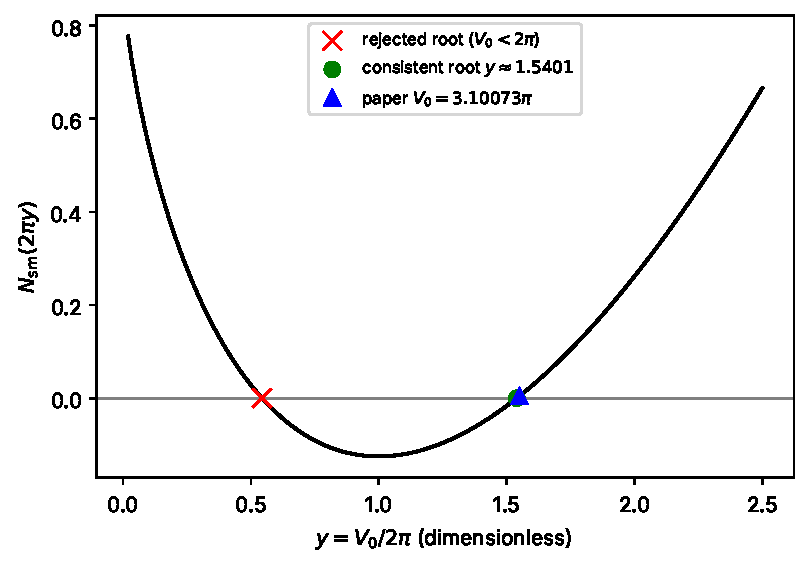
\includegraphics[width=0.85\linewidth]{figs/wu-sprung_v0func.pdf}
\caption{The function $\Nsm(2\pi y)=y\log y-y+\frac78$ against $y=V_0/2\pi$. It has two roots. The left one ($y<1$, i.e.\ $V_0<2\pi$) gives a well with $x(V)<0$ just above its bottom and is rejected (Eq.~\eqref{eq:wu-sprung-bottom}). The right root, $y\approx1.5401$ ($V_0\approx3.0803\pi$), is the consistent bottom; the paper's $V_0=3.10073\pi$ (marked) lies just beside it, where $\Nsm\approx0.0045$.}
\label{fig:wu-sprung-v0func}
\end{figure}

\begin{sample}{The harmonic bottom of the well}
Find the shape of the Wu--Sprung potential near $x=0$, with $V_0=3.10073\pi$.

\textbf{Step 1:} From \eqref{eq:wu-sprung-bottom}, $x\approx\frac{\sqrt{V-V_0}}{\pi}\log\frac{V_0}{2\pi}$.

\textbf{Step 2:} Solve for $V$: $V-V_0\approx\left(\dfrac{\pi x}{\log(V_0/2\pi)}\right)^2$.

\textbf{Step 3:} Numbers: $V_0/2\pi=1.550365$, $\log1.550365=0.43849$, $\pi/0.43849=7.1645$, squared $51.33$.

\[
\boxed{V(x)\approx V_0+51.3\,x^2\quad\text{near }x=0}
\]
The bottom is a harmonic well. This harmonic bottom is a by-product of the semiclassical construction. Only the lowest few levels are sensitive to it, and those are the levels for which Bohr--Sommerfeld, and hence the construction, is least accurate (the paper's maximum residual, $0.063$ spacings, occurs there).
\end{sample}

\begin{checkpoint}
Suppose the constant $\tfrac78$ in $\Nsm$ were replaced by $1$. What would happen to the consistency condition?
\end{checkpoint}
\checkanswer{It would become $f(y)=-1$, whose only solution is $y=1$, i.e.\ $V_0=2\pi$, the minimum of $f$. Then $\log(V_0/2\pi)=0$, the linear term of \eqref{eq:wu-sprung-bottom} vanishes and the bottom is no longer harmonic (Problem~7). The constant $\frac78$ genuinely shapes the well's floor.}

\begin{keyideas}
\item The natural consistency condition for $V_0$ is $\Nsm(V_0)=0$: no levels below the floor. Of its two roots, only the one with $V_0>2\pi$ gives a well with its minimum at $x=0$.
\item The root is $V_0\approx3.0803\pi$. The paper's $3.10073\pi$ is close to this root but not equal to it, and its exact origin is not derived here; it gives $\Nsm(V_0)\approx0.0045$, a uniform level shift of $0.0045$ spacings, Eq.~\eqref{eq:wu-sprung-phiws}.
\item Near the origin the well is harmonic, $V\approx V_0+51.3\,x^2$.
\end{keyideas}

%======================================================================
\section{The shape of the Wu--Sprung well}\label{sec:wu-sprung-shape}

\subsection{Growth at large $V$}

For large $V$, $a=\sqrt{V-V_0}$ and $b=\sqrt V$ are nearly equal. Rationalize the ratio in the second logarithm by multiplying top and bottom by $b+a$:
\[
\frac{b+a}{b-a}=\frac{(b+a)^2}{b^2-a^2}=\frac{(b+a)^2}{V_0}.
\]
For $V\gg V_0$, $b+a\approx2\sqrt V$, so $\frac{b+a}{b-a}\approx\frac{4V}{V_0}$. Also $a\approx b=\sqrt V$ in the first term. Then
\begin{equation}
x(V)\approx\frac{\sqrt V}{\pi}\left[\log\frac{V_0}{2\pi e^2}+\log\frac{4V}{V_0}\right]=\frac{\sqrt V}{\pi}\log\frac{2V}{\pi e^2}=\frac{\sqrt V}{\pi}\Bigl(\log\frac{2V}{\pi}-2\Bigr).
\label{eq:wu-sprung-asym}
\end{equation}
Note that $V_0$ has dropped out: far up the well, only the leading logarithmic growth of $\Nsm$ matters. The neglected terms come from $a=\sqrt V\bigl(1-V_0/2V+\cdots\bigr)$ and from the correction to $b+a$; they are smaller by a factor of order $V_0/V$.

So $x\sim\sqrt V\log V$: the chord grows a little faster than for the harmonic well ($x=\sqrt V$). Inverting roughly, $\sqrt V\approx\pi x/\log V$, and since $\log V\approx2\log x$ to leading order,
\[
V(x)\approx\left(\frac{\pi x}{2\log x}\right)^2\qquad(x\ \text{large, leading order}),
\]
so $V$ grows roughly like $(x/\log x)^2$: slower than harmonic by a factor $(\log x)^2$ (equivalently, the chord $x(V)$ is wider than the harmonic chord $\sqrt V$ by one logarithm). That matches the expectation of Section~\ref{sec:wu-sprung-target}: a density growing like $\log E$ needs a well that is softer than harmonic, but only logarithmically so.

\begin{figure}[htbp]\centering
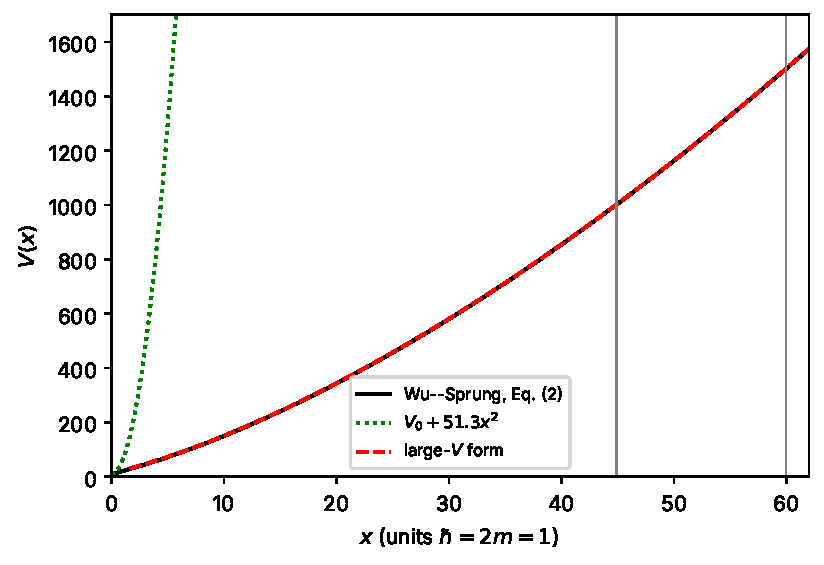
\includegraphics[width=0.85\linewidth]{figs/wu-sprung_potential.pdf}
\caption{The Wu--Sprung potential (solid), Eq.~\eqref{eq:wu-sprung-ws} inverted, for $0\le x\le 62$, with its harmonic bottom $V_0+51.3x^2$ (dotted) and the large-$V$ form from Eq.~\eqref{eq:wu-sprung-asym} (dashed). Vertical lines: the box half-widths $L=x(1000)=44.883$ (scale 1) and $L=x(1500)=59.957$ (scale 2) of the paper. Units $\hbar=2m=1$.}
\label{fig:wu-sprung-potential}
\end{figure}

\subsection{The box: $L=x(V_{\max})$}

A computer cannot handle the whole infinite line. The paper puts the well inside a box $[-L,L]$ with hard walls (Dirichlet conditions, Chapter~\ref{ch:bound-states}). The walls must be far enough out that the levels of interest never feel them; the natural choice is to place the wall where the potential reaches a chosen ceiling $V_{\max}$ well above those levels: $L=x(V_{\max})$.

\begin{sample}{The paper's two box sizes (RE3)}
Compute $L=x(1000)$ and $L=x(1500)$ from Eq.~\eqref{eq:wu-sprung-ws} with $V_0=3.10073\pi$.

\textbf{Step 1: constants.} $V_0=9.7412$, $\log\frac{V_0}{2\pi e^2}=0.43849-2=-1.56151$.

\textbf{Step 2: $V=1000$.} $a=\sqrt{990.259}=31.468$ and $b=31.623$. Their difference suffers from cancellation (Chapter~\ref{ch:asymptotics}), so compute it as $b-a=(b^2-a^2)/(b+a)=V_0/(b+a)=9.7412/63.091=0.1544$. Then $\frac{b+a}{b-a}=\frac{63.091}{0.1544}$, whose log is $6.0128$. So $\pi x=31.468(-1.5615)+31.623(6.0128)=-49.14+190.14=141.00$, and $x=141.00/\pi\approx44.88$.

\textbf{Step 3: precise evaluation} (carrying more digits, or with \texttt{qmnt.L\_of}): $x(1000)=44.883$, and in the same way $x(1500)=59.957$.

\textbf{Step 4: compare} with the asymptotic form \eqref{eq:wu-sprung-asym}: $\frac{\sqrt{1000}}{\pi}(\log\frac{2000}{\pi}-2)=44.855$, about $0.06\%$ low.

\[
\boxed{L_{\text{scale 1}}=44.883,\qquad L_{\text{scale 2}}=59.957}
\]
These are the paper's values (Sec.~II~B).
\end{sample}

Is $V_{\max}=1000$ high enough at scale 1? The paper scores the first 500 levels there, and $s_{500}\approx811$ (the true $t_{500}=811.18$, App.~A key anchors). A level at $E\approx811$ has its turning point inside the box, and its wavefunction decays exponentially (Chapter~\ref{ch:wkb}) in the forbidden region between the turning point and the wall, where $V$ climbs to $1000$. The wall affects such levels only through that exponentially small tail.

\subsection{Turning points: each level probes a place}

The turning point of level $n$ is the point where $V(x)=E_n$; since $E_n\approx s_n$ for this potential, it is
\begin{equation}
x_n=x(s_n).
\label{eq:wu-sprung-xn}
\end{equation}
In WKB the wavefunction amplitude is proportional to $(E-V)^{-1/4}$ (Chapter~\ref{ch:wkb}): large where the particle moves slowly, which is near the turning points. So $|\psi_n|^2$ is largest near $\pm x_n$, and a small change $\delta V$ near $x_n$ shifts level $n$ more than the same change elsewhere. In this sense \emph{each level probes the potential most strongly near its turning points}, and the map $n\mapsto x_n$ converts level indices into positions. This does not mean that level $n$ ignores the rest of the well: $|\psi_n|^2$ is spread over the whole allowed region $|x|<x_n$, so level $n$ feels a change anywhere inside its turning points, only less strongly. What level $n$ hardly feels is a change beyond $x_n$, where its wavefunction is exponentially small.

\begin{sample}{Where levels 201--300 turn}
Find the turning points of levels $201$ and $300$ of the Wu--Sprung well.

\textbf{Step 1: smooth zeros.} Solve $\Nsm(s)=n-\tfrac12$ by Brent's method: $s_{201}\approx398.3$ and $s_{300}\approx542.5$. Here is a quick check of the first value. We have $\Nsm(400)=63.66\log63.66-63.66+0.875\approx201.6$, which exceeds the target $200.5$ by about $1.1$. The level density there is $\Nsm'(400)=\log(63.66)/2\pi\approx0.661$, so $s_{201}$ lies about $1.1/0.661\approx1.7$ below $400$, consistent with $398.3$.

\textbf{Step 2: evaluate Eq.~\eqref{eq:wu-sprung-ws}.} $x(s_{201})\approx22.5$ and $x(s_{300})\approx28.5$.

\[
\boxed{\text{levels }201\text{--}300\text{ turn at }x\approx22.5\text{--}28.5}
\]
This agrees with the band $x=22.5$--$28.5$ that the paper's interpolation split (Sec.~III) quotes for the same levels.
\end{sample}

\begin{figure}[htbp]\centering
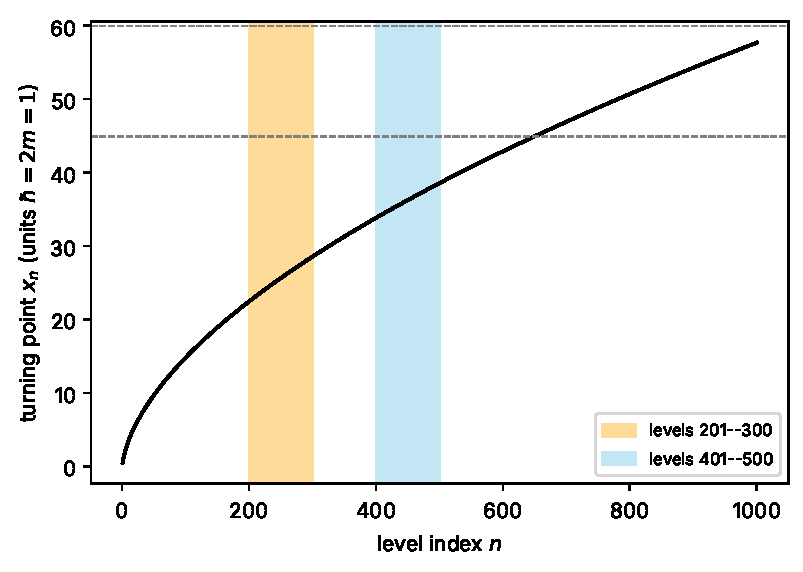
\includegraphics[width=0.85\linewidth]{figs/wu-sprung_turning.pdf}
\caption{The turning-point map $n\mapsto x_n=x(s_n)$ of the Wu--Sprung potential for $n=1,\dots,1000$. Shaded bands: levels 201--300 (the held-out gap of the paper's interpolation split) and levels 401--500 (the principal holdout RE5). Dashed lines: the box walls $L=44.883$ and $59.957$. Because the map is monotone, a band of levels corresponds to a band of positions.}
\label{fig:wu-sprung-turning}
\end{figure}

\begin{checkpoint}
A fitting algorithm changes $V$ only in the region $40<x<44$. Which levels of the scale-1 problem does this affect most?
\end{checkpoint}
\checkanswer{Those whose turning points $x_n$ lie in $40<x<44$. Since $x_n$ increases with $n$ and $x_{500}$ is about $38.5$ (Problem~10), these are levels above 500, which scale 1 does not score at all. A change there costs almost nothing on levels 1--500 (only through the exponentially small tails of their wavefunctions).}

\begin{keyideas}
\item For large $V$, $x(V)\approx\frac{\sqrt V}{\pi}(\log\frac{2V}{\pi}-2)$, Eq.~\eqref{eq:wu-sprung-asym}, so $V$ grows roughly like $(x/\log x)^2$: softer than harmonic by a factor $(\log x)^2$.
\item The box half-width is $L=x(V_{\max})$: $44.883$ for $V_{\max}=1000$, $59.957$ for $1500$.
\item Level $n$ turns at $x_n=x(s_n)$, where its wavefunction is largest; the monotone map $n\mapsto x_n$ links level index and position.
\end{keyideas}

%======================================================================
\section{Do the levels really sit on the smooth zeros?}\label{sec:wu-sprung-check}

We have made two approximations: Bohr--Sommerfeld, and the choice of $V_0$. Let us check them separately.

\textbf{Check 1: the semiclassical levels.} Using only the formula \eqref{eq:wu-sprung-ws}, compute the phase integral numerically, $\Phi(E)=2\int_0^{\sqrt{E-V_0}}x(E-u^2)\,\dd u$ (Eq.~\eqref{eq:wu-sprung-layer} after the substitution of Step E), and evaluate $\Phi(s_n)/\pi-(n-\tfrac12)$. Equation \eqref{eq:wu-sprung-phiws} predicts the constant $-\Nsm(V_0)\approx-0.0045$ for every $n$. A numerical evaluation with adaptive quadrature at $n=1,2,10,100,250,500$ confirms this to better than $10^{-6}$ (Problem~13 asks you to do all 500): by construction, the WKB levels of the Wu--Sprung well are the smooth zeros, shifted by $0.0045$ spacings.

\textbf{Check 2: the true quantum levels.} Bohr--Sommerfeld is itself an approximation. To test it we need the exact eigenvalues of $H$ in the box. We compute them with a method that is developed only later, in Chapter~\ref{ch:finite-differences}; here we use it as a black box and state exactly what we take on trust.
\begin{beyond}
\textbf{Finite differences, taken on trust (forward reference to Chapter~\ref{ch:finite-differences}).} We assume three facts proved there. (1) Sampling $V$ at $N$ equally spaced interior points $x_j$ of $(-L,L)$, with spacing $h=2L/(N+1)$ and $\psi=0$ at the walls, turns $H$ into a symmetric tridiagonal matrix with diagonal entries $2/h^2+V(x_j)$ and off-diagonal entries $-1/h^2$. Its lowest eigenvalues, found with \texttt{scipy.linalg.eigh\_tridiagonal} (Chapter~\ref{ch:eigen}), approximate the lowest levels of $H$ in the box. (2) For a fixed level, the error of the corresponding eigenvalue is of order $h^2$. (3) Hence the Richardson combination $E^{\rm Rich}=(4E_{h/2}-E_h)/3$ of results on grids of spacing $h$ and $h/2$ cancels the $h^2$ term. Note that this grid size $N$ is not the counting function $N(E)$ of Chapter~\ref{ch:wkb}; the paper uses the same letter for both.
\end{beyond}

\begin{pycode}
import numpy as np, qmnt
from scipy.linalg import eigh_tridiagonal
V0 = qmnt.V0
def xws(V):                                   # Eq. (2)
    a, b = np.sqrt(V - V0), np.sqrt(V)
    return (a*np.log(V0/(2*np.pi*np.e**2)) + b*np.log((b+a)/(b-a)))/np.pi
aa = np.linspace(0, np.sqrt(1200 - V0), 400001)
VV = V0 + aa**2                               # fine table of heights V
XX = np.concatenate([[0.0], xws(VV[1:])])     # and their x(V)
L = qmnt.L_of(1000)                   # 44.883
def levels(N, k=500):
    x = qmnt.grid(L, N); h = 2*L/(N+1)
    V = np.interp(np.abs(x), XX, VV)   # table lookup of V(x)
    d = 2/h**2 + V; e = -np.ones(N-1)/h**2
    return eigh_tridiagonal(d, e, select='i',
                            select_range=(0, k-1), eigvals_only=True)
Eh, Eh2 = levels(11999), levels(23999)  # h and h/2
ER = (4*Eh2 - Eh)/3                     # Richardson
n = np.arange(1, 501)
s = qmnt.smooth_zeros(n); g = qmnt.mean_gap(n)
dev = (ER - s)/g
print(np.mean(dev), np.max(np.abs(dev)))
\end{pycode}

\Cref{fig:wu-sprung-levels} shows the result. The exact levels track $s_n$ to a small fraction of a spacing over all 500 levels; the largest deviations are at the lowest $n$. That pattern is expected: Bohr--Sommerfeld is in general only asymptotically accurate, improving as $n$ grows (Chapter~\ref{ch:wkb}); the harmonic well is a special case where it is exact for every $n$. The paper reports the same comparison at scale 1 (Sec.~II~B): mean residual $0.005$ spacings, maximum $0.063$, ``worst at low $n$, the known semiclassical weakness of the construction''. We ran exactly the listing above, in which the potential is taken from a fine table of Eq.~\eqref{eq:wu-sprung-ws} and interpolated linearly onto the grid. Our run gives a signed mean deviation (the average of $(E_n-s_n)/\gap_n$, keeping its sign) of $0.004$ spacings and a maximum of $|E_n-s_n|/\gap_n$ of $0.05$ spacings, attained at the lowest levels. These are close to the paper's $0.005$ and $0.063$. The paper does not say whether its mean is signed or a mean of absolute values, and the last digits depend on details such as the interpolation between table points, so we compare only to the digits shown. Our signed mean is numerically close to the WKB offset $0.0045$ of Check~1.

The paper's mean of $0.005$ is not the same quantity as the WKB offset of $0.0045$ found in Check~1. The quantum deviation contains that uniform offset, but it also contains the genuine departures of the exact levels from Bohr--Sommerfeld, which are largest at low $n$. The two numbers are of similar size, but we do not claim that one explains the other.

\begin{figure}[htbp]\centering
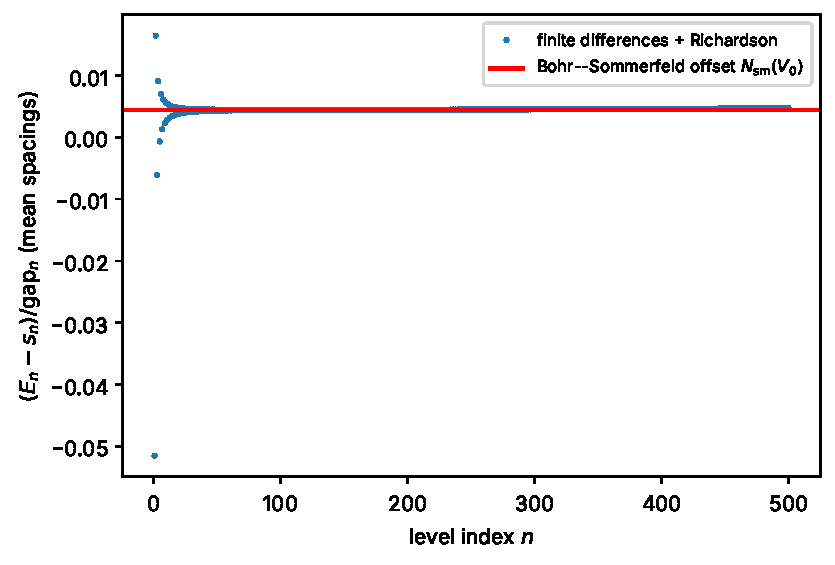
\includegraphics[width=0.85\linewidth]{figs/wu-sprung_levels.pdf}
\caption{Deviation of the levels of the Wu--Sprung well from the smooth zeros, $(E_n-s_n)/\gap_n$, for $n=1,\dots,500$ in the box $L=44.883$. Dots: Richardson-extrapolated finite-difference eigenvalues (grids of 11999 and 23999 interior points). Line: Bohr--Sommerfeld levels of the same potential, a constant offset $\Nsm(V_0)\approx0.0045$. The quantum levels differ from WKB mainly at low $n$.}
\label{fig:wu-sprung-levels}
\end{figure}

\begin{pitfall}
``The Wu--Sprung levels sit on the zeros'' is false. They sit on the \emph{smooth} zeros $s_n$. The true zeros $t_n$ differ from $s_n$ by fluctuations of typical size a quarter of a spacing (the null rms $0.263$ on zeros 401--500, RE5). The smooth well reproduces exactly the part of the zeros that a single formula, $\Nsm$, already knew.
\end{pitfall}

\begin{keyideas}
\item The WKB levels of the Wu--Sprung well are $s_n$ up to a uniform $0.0045$ spacings, an exact consequence of Eq.~\eqref{eq:wu-sprung-phiws}.
\item The exact quantum levels deviate by small fractions of a spacing, mostly at low $n$; the paper reports mean $0.005$, max $0.063$ spacings.
\item The well reproduces the smooth zeros, not the zeros: the fluctuations are not in it.
\end{keyideas}

%======================================================================
\section{Fluctuations, fractals and the empirical program}\label{sec:wu-sprung-empirical}

\subsection{What Wu and Sprung did next}

Having built the smooth well, Wu and Sprung \cite{wusprung} asked for more: a potential whose levels are the actual zeros $t_n$. They added a correction to the smooth potential and adjusted it until the low zeros were reproduced. They described the fitted potential as \emph{fractal}, hence the title of their paper ``Riemann zeros and a fractal potential''. That a potential reproducing the zeros must be irregular is plausible on general grounds: by the explicit formula (Chapter~\ref{ch:explicit-formula}) the fluctuations $t_n-s_n$ contain oscillations at every frequency $m\log p$ with slowly decaying amplitudes, and a potential that reproduces all of them must carry structure at many scales.

Later work continued the program. Van~Zyl and Hutchinson \cite{vanzyl} and Slater \cite{slater} extended the fractal fits; and Jaksch \cite{jaksch} generated successive zeros from a Wu--Sprung-type potential and traced the fractal corrections to the error of the Riemann--von Mangoldt approximation. Schumayer and Hutchinson \cite{schumayer} review this tradition. We describe these works only to the extent the paper does (its Sec.~I~A~a).

\subsection{The implicit logic and why it needs a test}

The paper states the implicit logic of this empirical program (Sec.~I): ``a potential reproducing many zeros accurately has captured something about the putative zeta operator.'' Recall from Chapter~\ref{ch:hilbert-polya} that the Hilbert--P\'olya conjecture (open) asks for a self-adjoint operator whose spectrum is the zeros. A fitted potential is a self-adjoint operator. If it reproduces 500 zeros, is it a candidate?

Count the ingredients. The smooth part is fixed by $\Nsm$ alone; we built it in this chapter from one formula and one constant. The fluctuating correction is adjusted to the data. If the correction has $M$ adjustable numbers and you fit $n$ levels, then when $M$ is large enough you can make the agreement as good as you like whether or not the potential ``knows'' anything. The paper finds in-sample rms $0.137$ spacings with $M=400$ on 400 zeros (Table~I) and below $10^{-4}$ spacings with $M=900$ on all 500 zeros (Sec.~III); the threshold is set by the coverage law of Chapter~\ref{ch:fitting}, not simply by $M=n$. A useful analogy, but only an analogy because fitting a potential is a nonlinear problem, is the linear result of Chapter~\ref{ch:least-squares}: an underdetermined linear fit has infinitely many exact solutions. Chapter~\ref{ch:generalization} develops the memorizing polynomial (RE4) in full. Agreement on the zeros used to build a model is therefore not evidence of structure. The test that can separate structure from capacity is to predict zeros the model was \emph{not} shown. This is exactly the question the paper puts to this program.

Two lessons of this chapter prepare that test.
\begin{enumerate}
\item \textbf{The null.} Before any fit, the Wu--Sprung well already predicts every level to within the fluctuations: its levels are $s_n$. Any fitted correction must beat ``predict $s_n$'', and the size of that target is the typical fluctuation (about $0.26$ spacings on zeros 401--500).
\item \textbf{Locality.} A correction $\delta V$ near position $x$ affects all levels whose turning points lie at or beyond $x$, most strongly those turning near $x$, and hardly at all the levels that turn well inside $x$, whose wavefunctions are exponentially small there (Section~\ref{sec:wu-sprung-shape}). Levels 1--400 all turn inside $|x|<x_{400}$, so they say almost nothing about $\delta V$ in the region $x_{400}<|x|<x_{500}$, which only higher levels reach. Conversely, a correction placed in a band of positions also shifts every level turning beyond that band, not only the levels turning inside it; this is why the paper's interpolation-split result (Sec.~III) is not as simple as ``each level controls its own patch''.
\end{enumerate}

\begin{checkpoint}
Why is it not a contradiction that the smooth Wu--Sprung potential has no fitted parameters at all (only $V_0$, fixed approximately by consistency), yet predicts the zeros with an rms error of about a quarter spacing?
\end{checkpoint}
\checkanswer{Because the information is in the target $\Nsm$, which was derived from the zeta function (Chapter~\ref{ch:counting-zeros}), not from fitting. The potential merely re-encodes $\Nsm$ as a well; it contains exactly the average behavior of the zeros, and the remaining quarter spacing is the fluctuation that $\Nsm$ does not describe.}

\begin{keyideas}
\item Wu and Sprung added fitted corrections to the smooth well and found fractal-looking structure; van Zyl--Hutchinson, Slater and Jaksch continued the program.
\item Fitting many zeros with many parameters shows capacity, not structure; the test is out-of-sample prediction against the null ``levels at $s_n$''.
\item The turning-point map tells you which part of the potential each level constrains: level $n$ feels changes anywhere inside its turning points, most strongly near them, and hardly any change beyond them.
\end{keyideas}

%======================================================================
\section{Paper connection}\label{sec:wu-sprung-paper}

\textbf{Eq.~(2), Sec.~II~B.} Our Eq.~\eqref{eq:wu-sprung-ws} is the paper's Eq.~(2), term for term, including the constant $V_0=3.10073\pi$ and the condition $V\ge V_0$. The paper's phrase ``defined implicitly'' means that Eq.~(2) gives $x$ as a function of $V$, and ``inverted pointwise by bracketed root finding'' (App.~A step 3: ``potential by Brent inversion of Eq.~(2) on a dense reference grid, cubic-spline interpolated'') is the inversion we discussed. The paper does not say how $V_0$ was obtained. Our Section~\ref{sec:wu-sprung-v0} gives the natural consistency condition $\Nsm(V_0)=0$, whose root is $3.0803\pi$; the paper's $3.10073\pi$ is close to but not equal to this root, and its exact origin is not derived here.

\textbf{The box, Sec.~II~B and App.~A step 3.} ``Scale 1 uses the domain $[-L,L]$ with $L=x(V{=}1000)=44.883$ and the first 500 levels scored; scale 2 extends to $L=x(V{=}1500)=59.957$ with 1000 levels.'' Sample Problem ``The paper's two box sizes'' reproduces both $L$ values from Eq.~(2). App.~A step 3 quotes them to more digits as $44.8827$ and $59.9572$.

\textbf{Accuracy of the construction, Sec.~II~B and App.~A key anchors.} The paper's statement that the Richardson levels match the smooth zeros to ``$0.005$ spacings mean, $0.063$ max (worst at low $n$, the known semiclassical weakness of the construction)'' is the comparison of \cref{fig:wu-sprung-levels}. The anchors give the same $0.005/0.063$ at scale 2. Our analysis adds one detail. With the paper's $V_0$, the WKB levels of the potential are offset uniformly by $\Nsm(V_0)\approx0.0045$ spacings. The published numbers do not let us separate how this offset combines with the non-WKB deviations in the paper's quoted mean.

\textbf{The null model, Sec.~II~C.} ``The null model is the unperturbed potential itself; numerically its holdout error coincides with that of the smooth zeros used as the oracle's null (both $0.2631$ on zeros 401--500).'' This chapter is why: the unperturbed Wu--Sprung levels are the smooth zeros to within a few thousandths of a spacing on average (the maximum deviation, $0.063$ in the paper and $0.05$ in our run, occurs at the lowest levels, far from the holdout 401--500), so ``predict the Wu--Sprung levels'' and ``predict $s_n$'' have the same error to the digits quoted. The paper correctly stresses that the two nulls are conceptually distinct (an eigenvalue spectrum versus the solution of the mean counting function); their numerical coincidence is a consequence of the construction derived here.

\textbf{Evenness of $\delta V$, Sec.~II~C ``Other bases''.} The paper fits only even corrections (cosine $\cos(k\pi x/L)$, Chebyshev $T_k(2|x|/L-1)$, hat functions in $|x|/L$). The paper does not state why it restricts to even corrections. A natural reading, from Section~\ref{sec:wu-sprung-inverse}, is that the semiclassical spectrum cannot distinguish left from right, so odd parts of $\delta V$ are not constrained by the levels. Evenness does not by itself make the fitted problem unique: the corrected potential need not be monotone, and the paper's point is precisely that many different $\delta V$ fit equally well.

\textbf{Turning points, Sec.~III interpolation split and Fig.~4.} ``Position maps to level index through the classical turning point, and levels 201--300 turn at $x=22.5$--$28.5$.'' This is our map \eqref{eq:wu-sprung-xn}. The Sample Problem ``Where levels 201--300 turn'' gives $22.5$--$28.5$, in agreement with the paper. Fig.~4(a),(b) of the paper shades exactly this band and shows that the fitted correction is largest there (rms $\delta V=40$ in the band, maximum $|\delta V|=199$ ``where the smooth potential is about $500$''). You can check the last remark with our formula. Across the band, $V(x)$ runs from about $398$ to about $543$, because the band lies between the turning points of $s_{201}\approx398.3$ and $s_{300}\approx542.5$.

\textbf{Sec.~V ($p=2$ period remark).} Sec.~V (paragraph ``The proposed mechanism fails quantitatively'') states that the $p=2$ oscillation, period $2\pi/\log2\approx9$ in $t$, is ``only $\sim$6--7 levels at these heights''; that conversion uses the mean spacing \eqref{eq:wu-sprung-gap} (Problem~14).

\textbf{Sec.~I and Sec.~I~A~a.} The paper's description of the empirical program (``Wu and Sprung showed that a smooth one-dimensional potential, fixed by the mean counting function, reproduces the low zeros after fitted fluctuating corrections; successors refined the reconstructions'') and its literature strand (a) are the subject of Section~\ref{sec:wu-sprung-empirical}. The paper's scope statement matters here: it tests only fluctuation potentials \emph{on the Wu--Sprung background} in three bases, and ``other backgrounds and other parametrizations \dots are not tested''. Its title says ``on the Wu--Sprung background'' for this reason.

\section{Summary}
% DYK-BEGIN
\begin{didyouknow}{A Fractal Well}
In 1993 Hua Wu and Donald Sprung published, in \emph{Physical Review E}, a one-dimensional potential whose lowest levels reproduce Riemann zeros. As they fitted more zeros, the correction to the smooth potential became rough and jagged, and they reported a fractal structure with dimension close to $1.5$. The fluctuations of the zeros had become fluctuations in the shape of the well.
\end{didyouknow}
% DYK-END

\begin{itemize}
\item Semiclassically, a single well's levels depend only on its width function, $\Phi(E)=\int_{V_0}^{E}w(V)\,\dd V/(2\sqrt{E-V})$, Eq.~\eqref{eq:wu-sprung-width}; evenness and monotonicity make the inverse problem unique, Eq.~\eqref{eq:wu-sprung-layer}.
\item The target $\Phi(E)=\pi\Nsm(E)$, Eq.~\eqref{eq:wu-sprung-match}, puts Bohr--Sommerfeld levels on the smooth zeros.
\item Abel inversion: $x(V)=\frac1\pi\int_{V_0}^{V}\Phi'(E)\,\dd E/\sqrt{V-E}$ if $\Phi(V_0)=0$, Eq.~\eqref{eq:wu-sprung-abel-inv}; the kernel integral is $\pi$, Eq.~\eqref{eq:wu-sprung-Kpi}.
\item The Wu--Sprung potential, Eq.~\eqref{eq:wu-sprung-ws} (paper Eq.~(2)), follows by exact integration.
\item The natural consistency condition for $V_0$ is $\Nsm(V_0)=0$ with $V_0>2\pi$: root $\approx3.0803\pi$. The paper's $3.10073\pi$ is close to but not equal to this root (its exact origin is not derived here) and shifts levels uniformly by $\approx0.0045$ spacings, Eq.~\eqref{eq:wu-sprung-phiws}.
\item Shape: harmonic bottom $V\approx V_0+51.3x^2$; $x\approx\frac{\sqrt V}\pi(\log\frac{2V}\pi-2)$ at large $V$, Eq.~\eqref{eq:wu-sprung-asym}; $L=44.883$ and $59.957$.
\item Turning-point map $x_n=x(s_n)$, Eq.~\eqref{eq:wu-sprung-xn}: levels 201--300 turn at $x\approx22.5$--$28.5$.
\item The well reproduces $s_n$, not $t_n$; fitted fluctuation corrections must be judged by held-out prediction against this null.
\end{itemize}

\section{Problems}

\begin{problemlist}
\prob{1}{For the linear well $V=|x|$ find the width function $w(V)$ and use Eq.~\eqref{eq:wu-sprung-width} to compute $\Phi(E)$. Compare with the Sample Problem on power-law wells.}
\prob{1}{Compute the mean spacing of the zeros at height $t=100$ from Eq.~\eqref{eq:wu-sprung-gap}.}
\prob{1}{Show directly from Eq.~\eqref{eq:wu-sprung-ws} that $x(V_0)=0$ for any $V_0>0$.}
\prob{2}{An infinite well $[-L,L]$ with $V=0$ inside has levels $(k\pi/2L)^2$ and $\Phi(E)=2L\sqrt E$. Apply the Abel inversion \eqref{eq:wu-sprung-abel-inv} with $V_0=0$ and interpret the result $x(V)=L$.}
\prob{2}{Differentiate Eq.~\eqref{eq:wu-sprung-xu} with Leibniz's rule to show $\dfrac{\dd x}{\dd V}=\dfrac{1}{2\pi a}\log\dfrac{V_0}{2\pi}+\dfrac1\pi\displaystyle\int_0^a\frac{\dd u}{V-u^2}$, and conclude that the Wu--Sprung potential is monotone for $x>0$ when $V_0>2\pi$.}
\prob{1}{Which of the two assumptions, evenness or monotonicity, removes the reflection ambiguity? Which removes multiple wells?}
\prob{2}{Replace $\frac78$ by $1$ in $\Nsm$. Show that the consistency condition forces $V_0=2\pi$ and find the leading behavior of $x(V)$ near the bottom. Is the bottom harmonic?}
\prob{2}{Using numpy and scipy, code Eq.~\eqref{eq:wu-sprung-ws} and compute $L=x(1000)$ and $x(1500)$. Compare with the paper's Sec.~II~B and with \texttt{qmnt.L\_of}.}
\prob{2}{(Paper, Sec.~III.) Compute the turning points $x(s_{201})$ and $x(s_{300})$ and compare with the paper's band $x=22.5$--$28.5$ for the held-out levels of the interpolation split.}
\prob{2}{Using qmnt, compute the turning points of levels 401 and 500 (the principal holdout, RE5). Which part of the scale-1 box do these levels probe?}
\prob{2}{(Paper, Sec.~II~C.) Explain why the paper can say that the null of the operator fits and the null of the arithmetic oracle coincide numerically ($0.2631$ on zeros 401--500), and why it still calls them conceptually distinct.}
\prob{3}{Derive Eq.~\eqref{eq:wu-sprung-asym} including the next correction: show that $x(V)=\frac{\sqrt V}{\pi}\bigl(\log\frac{2V}\pi-2\bigr)+\order\bigl(V^{-1/2}\log V\bigr)$.}
\prob{3}{Using scipy's \texttt{quad}, compute $\Phi(s_n)=2\int_0^{\sqrt{s_n-V_0}}x(s_n-u^2)\,\dd u$ for $n=1,\dots,500$ and show that $\Phi(s_n)/\pi-(n-\tfrac12)$ is the same constant for all $n$. Identify the constant.}
\prob{2}{(Paper, Sec.~V.) Show that one period $2\pi/\log2$ of the $p=2$ wave (RE2) corresponds to about 6--7 levels near $t=500$, as stated in the paper. (The paper's ``these heights'' refers to the training zeros 1--400, which span $t$ up to about $680$; check that the count stays between 6 and 7 there too.)}
\prob{2}{Construct a non-even potential with exactly the same Bohr--Sommerfeld levels as the Wu--Sprung well.}
\prob{3}{Show that for $\Phi(E)=cE^{\gamma}$ ($\gamma>0$, $V_0=0$) the Abel inversion gives $x(V)\propto V^{\gamma-1/2}$, and find the proportionality constant in terms of $\int_0^{\pi/2}\sin^{2\gamma-1}\varphi\,\dd\varphi$.}
\prob{3}{Use the Abel inversion to recover the linear well from $\Phi(E)=\frac43E^{3/2}$.}
\prob{2}{(Paper, Sec.~I.) In a paragraph, explain why reproducing the first 500 zeros with a 900-coefficient correction to the Wu--Sprung well is not, by itself, evidence for the Hilbert--P\'olya conjecture.}
\prob{1}{Compute $\Nsm(t_1)$ for $t_1=14.134725$ (RE1). Is it close to $\frac12$, as Eq.~\eqref{eq:wu-sprung-sn} would suggest for $n=1$?}
\prob{3}{Using numpy and scipy, reproduce \cref{fig:wu-sprung-levels} at the smaller grid pair $N=5999$ and $11999$. Does Richardson extrapolation still bring the levels within a small fraction of a spacing of $s_n$?}
\end{problemlist}

\section{Answers to selected problems}

\textbf{1.} $x_\pm=\pm V$, so $w=2V$. Then $\Phi=\int_0^E\frac{2V\,\dd V}{2\sqrt{E-V}}$; with $V=E-u^2$ this is $2\int_0^{\sqrt E}(E-u^2)\dd u=2(E^{3/2}-E^{3/2}/3)=\frac43E^{3/2}$, matching $2I_1E^{3/2}$ with $I_1=\frac23$.

\textbf{2.} $100/2\pi=15.9155$ and $\log15.9155=2.7673$, so $\gap=2\pi/2.7673=2.2705$.

\textbf{3.} At $V=V_0$, $a=0$: the first term is $0$ and the second is $\sqrt{V_0}\log(\sqrt{V_0}/\sqrt{V_0})=0$.

\textbf{5.} From \eqref{eq:wu-sprung-xu}, $x=\frac1\pi\int_0^a\log\frac{V-u^2}{2\pi}\dd u$ with $a=\sqrt{V-V_0}$, $\dd a/\dd V=1/(2a)$. Leibniz: the boundary term is $\frac1\pi\log\frac{V-a^2}{2\pi}\cdot\frac1{2a}=\frac1{2\pi a}\log\frac{V_0}{2\pi}$, and $\partial_V\log(V-u^2)=1/(V-u^2)$. For $V_0>2\pi$ both terms are positive (the integrand $1/(V-u^2)>0$ since $u\le a<\sqrt V$), so $x$ increases with $V$ and the inverse $V(x)$ increases with $x$.

\textbf{6.} Evenness removes reflection (and translation). Monotonicity on $x>0$ ensures a single well, so each height has one chord.

\textbf{7.} $f(y)=y\log y-y=-1$ has the unique solution $y=1$ (the minimum of $f$), so $V_0=2\pi$. Then $\log\frac{V_0}{2\pi e^2}=-2$ and, with $\log\frac{1+r}{1-r}=2r+\frac23r^3+\cdots$, $\pi x=-2a+2a+\frac{2a^3}{3V_0}+\cdots$, so $x\approx\frac{2a^3}{3\pi V_0}$. Hence $V-V_0=a^2\propto x^{2/3}$: a cusp at the bottom, not harmonic.

\textbf{9.} $s_{201}\approx398.3$ and $s_{300}\approx542.5$ give $x(s_{201})\approx22.5$ and $x(s_{300})\approx28.5$. This agrees with the paper's $22.5$--$28.5$.

\textbf{11.} The unperturbed Wu--Sprung levels equal $s_n$ to within a few thousandths of a spacing on average (Sec.~\ref{sec:wu-sprung-check}; the largest deviations, a few hundredths, occur at the lowest levels, not in the holdout), so the error of predicting them for $t_n$ equals the error of predicting $s_n$, to the digits shown. Conceptually one is an eigenvalue list of a particular operator, the other the solution of $\Nsm(s)=n-\frac12$; they coincide only because the Wu--Sprung construction was designed to make them coincide, and the coincidence is approximate.

\textbf{13.} The constant is $-\Nsm(V_0)\approx-0.0045$ for $V_0=3.10073\pi$, by Eq.~\eqref{eq:wu-sprung-phiws}; numerically it is the same for all $n$ to quadrature accuracy.

\textbf{15.} Keep the width $2x(V)$ but share it unequally: for $0<\beta<1$ set $x_+(V)=(1+\beta)x(V)$ and $x_-(V)=-(1-\beta)x(V)$, i.e.\ $\tilde V(x)=V_{\rm WS}(x/(1+\beta))$ for $x\ge0$ and $V_{\rm WS}(x/(1-\beta))$ for $x<0$. Chords have length $2x(V)$, so by Eq.~\eqref{eq:wu-sprung-width} the Bohr--Sommerfeld levels are unchanged.

\textbf{17.} $\Phi'=2\sqrt E$, so $x=\frac2\pi\int_0^V\sqrt{E}\,\dd E/\sqrt{V-E}$. With $E=V\sin^2\varphi$, $\dd E=2V\sin\varphi\cos\varphi\,\dd\varphi$, the integral is $\int_0^{\pi/2}2V\sin^2\varphi\,\dd\varphi=\pi V/2$. Hence $x=V$, i.e.\ $V=|x|$.

\textbf{19.} $t_1/2\pi=2.24961$ and $\log2.24961=0.81076$, so $\Nsm=2.24961\times0.81076-2.24961+0.875=0.449$. This is close to $\frac12$. Because $\Nsm$ is increasing and $\Nsm(t_1)<\Nsm(s_1)=\frac12$, we have $t_1<s_1$. The difference $\frac12-0.449\approx0.05$ means that the first zero lies about $0.05$ of a mean spacing below $s_1$.
